% recurrence.tex
% Updated January 11, 2012

\chapter{Recurrence Equations}\label{ch:recurrence}

We have already seen many examples of recurrence in the definitions of
combinatorial functions and expressions. The development of number
systems in \autoref{app:background} lays the groundwork for recurrence in
mathematics. Other examples we have seen include the Collatz sequence
of \hyperref[ex:collatz]{Example~\ref*{ex:collatz}} and the binomial
coefficients. In \autoref{ch:induction}, we also saw how recurrences
could arise when enumerating strings with certain restrictions, but we
didn't discuss how we might get from a recursive definition of a
function to an explicit definition depending only on $n$, rather than
earlier values of the function. In this chapter, we present a more
systematic treatment of recurrence with the end goal of finding closed
form expressions for functions defined recursively---whenever
possible.  We will focus on the case of linear recurrence
equations. At the end of the chapter, we will also revisit some of
what we learned in \autoref{ch:genfunction} to see how generating
functions can also be used to solve recurrences.

\section{Introduction}\label{s:recurrence:intro}

\subsection{Fibonacci numbers}\label{s:recurrence:intro:fib}
One of the most well-known recurrences arises from a simple
story. Suppose that a scientist introduces a pair of newborn rabbits
to an isolated island. This species of rabbits is unable to reproduce
until their third month of life, but after that produces a new pair of
rabbits each month. Thus, in the first and second months, there is one
pair of rabbits on the island, but in the third month, there are two
pairs of rabbits, as the first pair has a pair of offspring. In the
fourth month, the original pair of rabbits is still there, as is their
first pair of offspring, which are not yet mature enough to
reproduce. However, the original pair gives birth to another pair of
rabbits, meaning that the island now has three pairs of
rabbits. Assuming that there are no rabbit-killing predators on the
island and the rabbits have an indefinite lifespan, how many pairs of
rabbits are on the island in the tenth month?

Let's see how we can get a recurrence from this story. Let $f_n$
denote the number of pairs rabbits on the island in month $n$. Thus,
$f_1 = 1$, $f_2 = 1$, $f_3=2$, and $f_4=3$ from our account above. How
can we compute $f_n$? Well, in the $n^\text{th}$ month we have all the
pairs of rabbits that were there during the previous month, which is
$f_{n-1}$; however, some of those pairs of rabbits also reproduce
during this month. Only the ones who were born prior to the previous
month are able to reproduce during month $n$, so there are $f_{n-2}$
pairs of rabbits who are able to reproduce, and each produces a new
pair of rabbits. Thus, we have that the number of rabbits in month $n$
is $f_n = f_{n-1} + f_{n-2}$ for $n\geq 3$ with $f_1=f_2=1$. The
sequence of numbers $\{f_n\colon n\geq 0\}$ (we take $f_0=0$, which
satisfies our recurrence) is known as the \emph{Fibonacci sequence}
after Leonardo of Pisa, better known as Fibonacci, an Italian
mathematician who lived from about 1170 until about 1250. The terms
$f_0,f_1,\dots,f_{20}$ of the Fibonacci sequence are
\[
0,1,1,2,3,5,8,13,21,34,55,89,144,233,377,610,987, 1597,2584,4181,6765.
\]
Thus, the answer to our question about the number of pairs of rabbits
on the island in the tenth month is $55$. That's really easy to
compute, but what if we asked for the value of $f_{1000}$ in the
Fibonacci sequence? Could you even tell whether the following
inequality is true or false---without actually finding $f_{1000}$?
\[
f_{1000} < 232748383849990383201823093383773932
\]
% \noindent
% \textbf{Extra Credit.}\quad Modify the code for \texttt{big\_integer\_addition.c}
% to calculate $f_{1000}$ in the Fibonacci
% sequence.  Turn in your solutions as two files, the first being
% the source code, and the second the output for the value of $f_{1000}$
% using the syntax of the \texttt{big\_integer\_addition.c}.

Consider the sequence $\{f_{n+1}/f_n:n\ge1\}$ of ratios of consecutive
terms of the Fibonacci sequence. \autoref{tab:fib-ratios} shows these
ratios for $n\geq 18$.
\begin{table}
\begin{align*}
1/1 &= 1.0000000000\\
2/1 &= 2.0000000000\\
3/2 &= 1.5000000000\\
5/3 &= 1.6666666667\\
8/5 &= 1.6000000000\\
13/8 &= 1.6250000000\\
21/13 &= 1.6153846154\\
34/21 &= 1.6190476190\\
55/34 &= 1.6176470588\\
89/55 &= 1.6181818182\\
144/89 &= 1.6179775281\\
233/144 &= 1.6180555556\\
377/233 &= 1.6180257511\\
610/377 &= 1.6180371353\\
987/610 &= 1.6180327869\\
1597/987 &= 1.6180344478\\
2584/1597 &= 1.6180338134\\
4181/2584 &= 1.6180340557
\end{align*}
\caption{The ratios $f_{n+1}/f_{n}$ for $n\leq 18$\label{tab:fib-ratios}}
\end{table}
The ratios seem to be converging to a number.  Can we determine this
number? Does this number have anything to do with an explicit formula
for $f_n$ (if one even exists)?

\begin{example}
  The Fibonacci sequence would not be as well-studied as it is if it
  were only good for counting pairs of rabbits on a hypothetical
  island. Here's another instance which again results in the Fibonacci
  sequence.  Let $c_n$ count the number of ways a $2\times n$
  checkerboard can be covered by $2\times 1$ tiles.  Then $c_1=1$ and
  $c_2=2$ while the recurrence is just $c_{n+2} = c_{n+1}+c_n$, since
  either the rightmost column of the checkerboard contains a vertical
  tile (and thus the rest of it can be tiled in $c_{n+1}$ ways) or the
  rightmost two columns contain two horizontal tiles (and thus the
  rest of it can be tiled in $c_n$ ways).
\end{example}


\subsection{Recurrences for strings}\label{s:recurrence:intro:strings}
In \autoref{ch:induction}, we saw several times how we could  find
recurrences that gave us the number of binary or ternary strings of
length $n$ when we place a restriction on certain patterns appearing
in the string. Let's recall a couple of those types of questions in
order to help generate more recurrences to work with.

\begin{example}\label{ex:recurrence:binary-strings-no-11}
Let $a_{n}$ count the number of binary strings of length $n$
in which no two consecutive characters are~$1$'s.  Evidently,
$a_1=2$ since both binary strings of length~$1$ are ``good.''  Also,
$a_2=3$ since only one of the four binary strings of length~$2$ is
``bad,'', namely $(1,1)$. And $a_3= 5$, since of the $8$ binary
strings of length~$3$, the following three strings are ``bad'':
\[
(1,1,0), (0,1,1), (1,1,1).  
\]
More generally, it is easy to see that the sequence satisfies the
recurrence $a_{n+2} = a_{n+1}+a_n$, since we can partition the set of
all ``good'' strings into two sets, those ending in $0$ and those
ending in~$1$.  If the last bit is~$0$, then in the first $n+1$
positions, we can have any ``good'' string of length~$n+1$.  However,
if the last bit is~$1$, then the preceding bit must be $0$, and then
in the first $n$ positions we can have any ``good'' string of
length~$n$.

As a result, this sequence is just the Fibonacci numbers, albeit
offset by~$1$ position, i.e, $a_{n} = f_{n+1}$.
\end{example}

\begin{example}\label{ex:recurrence:ternary-strings-no-20}
  Let $t_n$ count the number of ternary strings in which we never have
  $(2,0)$ occuring as a substring in two consecutive positions.  Now
  $t_1=3$ and $t_2=8$, as of the $9$ ternary strings of length~$2$,
  exactly one of them is ``bad.''  Now consider the set of all good
  strings grouped according to the last character.  If this character
  is a $2$ or a $1$, then the preceding $n+1$ characters can be any
  ``good'' string of length~$n+1$.  However, if the last character is
  a $0$, then the first $n+1$ characters form a good string of length
  ~$n+1$ which does not end in a~$2$.  The number of such strings is
  $t_{n+1} - t_n$.  Accordingly, the recurrence is $t_{n+2} = 3t_{n+1}
  - t_n$.  In particular, $t_3 = 21$.
\end{example}

\subsection{Lines and regions in the plane}\label{s:recurrence:intro:lines}
Our next example takes us back to one of the motivating problems
discussed in \autoref{ch:intro}.  In \autoref{fig:geomregions}, we
show a family of $4$ lines in the plane.  Each pair of lines
intersects and no point in the plane belongs to more than two lines.
These lines determine~$11$ regions.  We ask
 \begin{figure}
 \begin{center}
 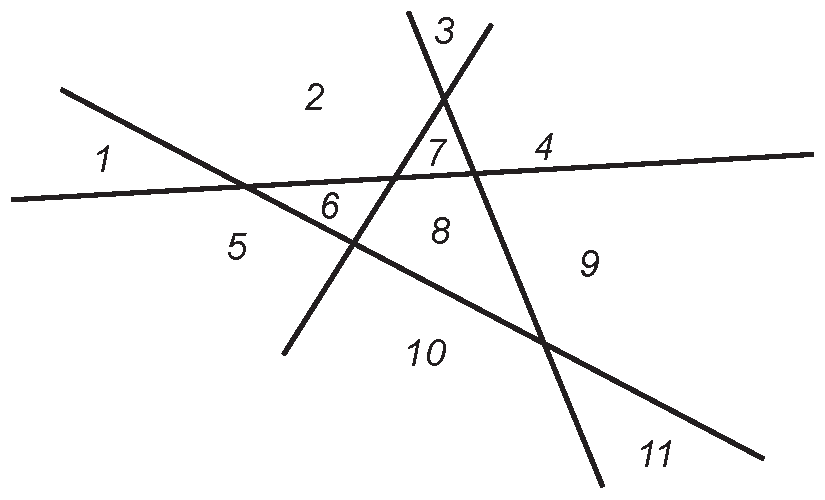
\includegraphics[scale=.6]{recurrence-figs/3012-fig9}\\
 \caption{\label{fig:geomregions}Lines and Regions} 
 \end{center}
 \end{figure}
how many regions a family of $1000$ lines would determine, given
these same restrictions on how the lines intersect.  More generally, let
$r_n$ denote the number of regions determined by $n$ lines.  Evidently,
$r_1=2$, $r_2=4$, $r_3=7$ and $r_4=11$.  Now it is easy to see that
we have the recurrence $r_{n+1} = r_n+n+1$.  To see this, choose any
one of the $n+1$ lines and call it $l$.  Line $l$ 
intersects each of the other lines and since no point in the plane
belongs to three or more lines, the points where $l$ intersects
the other lines are distinct.  Label them consecutively as
$x_1,x_2,\dots,x_n$.  Then these points divide line $l$ into
$n+1$ segments, two of which (first and last) are infinite.  Each of
these segments partitions one of the regions determined by the other
$n$ lines into two parts, meaning we have the $r_n$ regions determined
by the other $n$ lines and $n+1$ new regions that $l$ creates.

\section{Linear Recurrence Equations}\label{s:recurrence:linear}

What do all of the examples of the previous section have in common?
The end result that we were able to achieve is a \emph{linear
  recurrence}, which tells us how we can compute the $n^\text{th}$
term of a sequence given some number of previous values (and perhaps
also depending nonrecursively on $n$ as well, as in the last example).
More precisely a recurrence equation is said to be \textit{linear}
when it has the following form
\[
c_0a_{n+k}+ c_1a_{n+k-1} + c_2a_{n+k-2} + \dots+c_ka_{n} = g(n),
\] 
where $k\ge1$ is an integer, $c_0,c_1,\dots,c_k$ are constants with
$c_0,c_k\neq0$, and
$g:\ints\rightarrow\reals$ is a function. (What we have just defined
may more properly be called a linear recurrence equation with
\emph{constant coefficients}, since we require the $c_i$ to be
constants and prohibit them from depending on $n$. We will avoid this
additional descriptor, instead choosing to speak of linear recurrence
equations with \emph{nonconstant coefficients} in case we allow the
$c_i$ to be functions of $n$.) A linear equation is
\textit{homogeneous} if the function $g(n)$ on the right hand side
is the zero function.  For example, the Fibonacci sequence satisfies
the homogeneous linear recurrence equation
\[
a_{n+2} - a_{n+1} - a_n = 0.
\]
Note that in this example, $k=2$, $c_0=1$ and $c_k=-1$.

As a second example, the ternary sequence in
\hyperref[ex:recurrence:ternary-strings-no-20]{Example~\ref*{ex:recurrence:ternary-strings-no-20}}
  satifies the  homogeneous linear recurrence equation
\[
t_{n+2} - 3t_{n+1} + t_n = 0.
\]
Again, $k=2$ with $c_0=c_k=1$.

On the other hand, the sequence $r_n$ defined in
\autoref{s:recurrence:intro:lines} satisfies the nonhomogeneous
linear recurrence equation
\[
r_{n+1} - r_{n} = n+1.
\]
In this case, $k=1$, $c_0=1$ and $c_k=-1$.

Our immediate goal is to develop techniques for solving linear
recurrence equations of both homogeneous and nonhomogeneous types. We
will be able to fully resolve the question of solving homogeneous
linear recurrence equations and discuss a sort of ``guess-and-test''
method that can be used to tackle the more tricky nonhomogeneous type.

\section{Advancement Operators}\label{s:recurrence:adv-ops}

Much of our motivation for solving recurrence equations comes from an
analogous problem in continuous mathematics---differential
equations. You don't need to have studied these beasts before in order
to understand what we will do in the remainder of this chapter, but if
you have, the motivation for how we tackle the problems will be
clearer. As their name suggests, differential equations involve
derivatives, which we will denote using ``operator'' notation by $Df$
instead of the Leibniz notation $df/dx$. In our notation, the second
derivative is $D^2 f$, the third is $D^3 f$, and so on. Consider the
following example.

\begin{example}\label{ex:recurrence:diffeq}
  Solve the equation
  \[Df = 3f\] if $f(0) = 2$. Even if you've not studied differential
  equations, you should recognize that this question is really just
  asking us to find a function $f$ such that $f(0)=2$ and its
  derivative is three times itself. Let's ignore the \emph{initial
    condition} $f(0)=2$ for the moment and focus on the meat of the
  problem. What function, when you take its derivative, changes only
  by being multiplied by $3$?  You should quickly think of the
  function $e^{3x}$, since $D(e^{3x}) = 3e^{3x}$, which has exactly
  the property we desire. Of course, for any constant $c$, the
  function $ce^{3x}$ also satisfies this property, and this gives us
  the hook we need in order to satisfy our initial condition. We have
  $f(x) = ce^{3x}$ and want to find $c$ such that $f(0)=2$. Now $f(0)
  = c\cdot 1$, so $c=2$ does the trick and the solution to this very
  simple differential equation is $f(x) = 2e^{3x}$.
\end{example}

With differential equations, we apply the differential operator $D$ to
differentiable (usually infinitely differentiable) functions. For
recurrence equations, we consider the vector space $V$ whose elements
are functions from the set $\mathbb{Z}$ of integers to the set
$\mathbb{C}$ of complex numbers.  We then consider a function
$A:V\longrightarrow V$, called the 
\textit{advancement operator}, and defined by $A f(n) = f(n+1)$
(By various tricks and sleight of hand, we can extend a sequence 
$\{a_n\colon n\geq n_0\}$ to be a function whose domain is all of $\ints$, 
so this technique will apply to our problems). 
More generally, $A^p f(n)= f(n+p)$ when $p$ is
a positive integer.

\begin{example}
Let $f\in V$ be defined by $f(n)=7n-9$.  Then we apply the advancement
operator polynomial $3A^2-5A+4$ to $f$ with $n=0$ as follows:
\[
(3A^2-5A+4)f(0)=3f(2) - 5f(1) +4f(0)= 3(5)-5(-2)+4(-9)=-11.
\]
\end{example}

As an analogue of
\hyperref[ex:recurrence:diffeq]{Example~\ref*{ex:recurrence:diffeq}},
consider the following simple example involving the advancement
operator.

\begin{example}\label{ex:recurrence:adveq}
  Suppose that the sequence $\{s_n\colon n\geq 0\}$ satisfies $s_0 =
  3$ and $s_{n+1} = 2s_{n}$ for $n\geq 1$. Find an explicit formula
  for $s_n$.

  First, let's write the question in terms of the advancement
  operator. We can define a function $f(n) = s_n$ for $n\geq 0$, and
  then the information given becomes that $f(0)=3$ and
  \[Af(n) = 2f(n),\qquad n\geq 0.\]
  What function has the property that when we advance it, i.e.,
  evaluate it at $n+1$, it gives twice the value that it takes at $n$?
  The first function that comes into your mind should be $2^n$. Of
  course, just like with our differential equation, for any constant
  $c$, $c2^n$ also has this property. This suggests that if we take
  $f(n) = c2^n$, we're well on our way to solving our problem. Since
  we know that $f(0) = 3$, we have $f(0) = c2^0 = c$, so $c=
  3$. Therefore, $s_n = f(n) = 3\cdot 2^n$ for $n\geq 0$. This clearly
  satisfies our initial condition, and now we can check that it also
  satisfies our advancement operator equation:
  \[Af(n) = 3\cdot 2^{n+1} = 3\cdot 2\cdot 2^n = 2\cdot (3\cdot 2^n) =
  2\cdot f(n).\]
\end{example}

Before moving on to develop general methods for solving advancement
operator equations, let's say a word about why we keep talking in
terms of operators and mentioned that we can view any sequence as a
function with domain $\ints$. If you've studied any linear algebra, you
probably remember learning that the set of all
infinitely-differentiable functions on the real line form a vector
space and that differentiation is a linear operator on those
functions. Our analogy to differential equations holds up just fine
here, and functions from $\ints$ to $\mathbb{C}$ form a vector space and $A$ is a
linear operator on that space. We won't dwell on the technical aspects
of this, and no knowledge of linear algebra is required to understand
our development of techniques to solve recurrence equations. However,
if you're interested in more placing everything we do on rigorous
footing, we discuss this further in \autoref{s:recurrence:rigorous}.

\subsection{Constant Coefficient Equations}\label{s:recurrence:adv-ops:const-coeff}

It is easy to see that a linear recurrence equation can be
conveniently rewritten using a polynomial $p(A)$ of the 
advancement operator:
\begin{equation}\label{eqn:advance}
p(A)f=(c_0A^{k}+ c_1A^{k-1} + c_2A^{k-2} + \dots+c_k)f = g.
\end{equation} 
In equation~\ref{eqn:advance}, we intend that $k\ge1$ is an integer,
$g$ is a fixed vector (function) from $V$, and $c_0,c_1,\dots,
c_k$ are constants with $c_0,c_k\neq0$.  Note that since $c_0\neq0$,
we can divide both sides by $c_0$, i.e., we may in fact assume
that $c_0=1$ whenever convenient to do so.

\subsection{Roots and Factors}\label{s:recurrence:adv-ops:roots-factors}

The polynomial $p(A)$ can be analyzed like any other polynomial.
It has roots and factors, and although these may be difficult to
determine, we know they exist.  In fact, if the degree of $p(A)$ 
is $k$, we know that over the field of complex numbers, $p(A)$
has $k$ roots, counting multiplicities.  Note that since we assume
that $c_k\neq0$, all the roots of the polynomial $p$ are non-zero.

\subsection{What's Special About Zero?}\label{s:recurrence:adv-ops:zero}

Why have we limited our attention to recurrence equations of the form
$p(A)f = g$ where the constant term in $p$ is non-zero?  Let's
consider the alternative for a moment.  Suppose that the constant term
of $p$ is zero and that $0$ is a root of $p$ of multiplicity $m$.
Then $p(A) = A^mq(A)$ where the constant term of $q$ is non-zero.  And
the equation $p(A)f=g$ can then be written as $A^mq(A)f=g$.  To solve
this equation, we consider instead the simpler problem $q(A)f=g$.
Then $h$ is a solution of the original problem if and only if the
function $h'$ defined by $h'(n) = h(n+m)$ is a solution to the simpler
problem.  In other words, solutions to the original problem are just
translations of solutions to the smaller one, so we will for the most
part continue to focus on advancement operator equations where $p(A)$
has nonzero constant term, since being able to solve such problems is
all we need in order to solve the larger class of problems.

As a special case, consider the equation $A^m f =g$.  This requires
$f(n+m)=g(n)$, i.e., $f$ is just a translation of $g$.

\section{Solving advancement operator
  equations}\label{s:recurrence:solving}

In this section, we will explore some ways of solving advancement
operator equations. Some we will make up just for the sake of solving,
while others will be drawn from the examples we developed in
\autoref{s:recurrence:intro}. Again, readers familiar with
differential equations will notice many similarities between the
techniques used here and those used to solve linear differential
equations with constant coefficients, but we will not give any further
examples to make those parallels explicit.

\subsection{Homogeneous equations}\label{s:recurrence:solving:homogeneous}

Homogeneous equations, it will turn out, can be solved using very
explicit methodology that will work any time we can find the roots of
a polynomial. Let's start with another fairly straightforward example.

\begin{example}\label{ex:recurrence:deg2}
  Find all solutions to the advancement operator equation
  \begin{equation}(A^2+A-6)f = 0.\label{eqn:recurrence:deg2}\end{equation}

  Before focusing on finding \emph{all} solutions as we've been asked
  to do, let's just try to find \emph{some} solution. We start by noticing
  that here $p(A) = A^2+A-6 = (A+3)(A-2)$. With $p(A)$ factored like
  this, we realize that we've already solved part of this problem in
  \hyperref[ex:recurrence:adveq]{Example~\ref*{ex:recurrence:adveq}}!
  In that example, the polynomial of $A$ we encountered was (while not
  explicitly stated as such there) $A-2$. The solutions to $(A-2)f_1=0$
  are of the form $f_1(n) = c_12^n$. What happens if we try such a
  function here? We have
  \[(A+3)(A-2)f_1(n) = (A+3)0 = 0,\]
  so that $f_1$ is a solution to our given advancement operator
  equation. Of course, it can't be \emph{all} of them. However, it's
  not hard to see now that $(A+3)f_2 = 0$ has as a solution $f_2(n) =
  c_2(-3)^n$ by the same reasoning that we used in
  \hyperref[ex:recurrence:adveq]{Example~\ref*{ex:recurrence:adveq}}. Since
  $(A+3)(A-2) = (A-2)(A+3)$, we see right away that $f_2$ is also a
  solution of \autoref{eqn:recurrence:deg2}.

  Now we've got two infinite families of solutions to
  \autoref{eqn:recurrence:deg2}. Do they give us \emph{all} the
  solutions? It turns out that by combining them, they do in fact give
  all of the solutions. Consider what happens if we take $f(n) = c_1
  2^n + c_2 (-3)^n$ and apply $p(A)$ to it. We have
  \begin{align*}
    (A+3)(A-2)f(n) & = (A+3)(c_1 2^{n+1} + c_2 (-3)^{n+1} - 2(c_12^n +
    c_2(-3)^n))\\
    & = (A+3)(-5c_2(-3)^{n})\\
    & = -5c_2(-3)^{n+1}-15c_2(-3)^n\\
    & = 15c_2(-3)^n - 15c_2(-3)^n\\
    &=0.
  \end{align*}
  It's not all that hard to see that since $f$ gives a two-parameter family of
  solutions to \autoref{eqn:recurrence:deg2}, it gives us all the
  solutions, as we will show in detail in \autoref{s:recurrence:rigorous}.
\end{example}

What happened in this example is far from a fluke. If you have an
advancement operator equation of the form $p(A)f=0$ (the constant term
of $p$ nonzero) and $p$ has degree $k$, then the \emph{general
  solution} of $p(A)f=0$ will be a $k$-parameter family (in the
previous example, our parameters are the constants $c_1$ and $c_2$)
whose terms come from solutions to simpler equations arising from the
factors of $p$. We'll return to this thought in a little bit, but
first let's look at another example.

\begin{example}\label{ex:recurrence:ternary-strings-no-20-solved}
  Let's revisit the problem of enumerating ternary strings of length
  $n$ that do have $(2,0)$ occurring as a substring in two consecutive
  positions that we encountered in
  \hyperref[ex:recurrence:ternary-strings-no-20]{Example~\ref*{ex:recurrence:ternary-strings-no-20}}. There
  we saw that this number satisfies the recurrence equation
  \[t_{n+2} = 3t_{n+1} - t_n,\qquad n\geq 1\]
  and $t_1 = 3$ and $t_2=8$. Before endeavoring to solve this, let's
  rewrite our recurrence equation as an advancement operator
  equation. This gives us
  \begin{equation}
    \label{eqn:recurrence:ternary}
    p(A)t=(A^2-3A+1)t=0.
  \end{equation}
  The roots of $p(A)$ are $(3\pm\sqrt{5})/2$. Following the approach
  of the previous example, our general solution is
  \[t(n) = c_1\left(\frac{3+\sqrt{5}}{2}\right)^n +
  c_2\left(\frac{3-\sqrt{5}}{2}\right)^n.\]
  This probably looks suspicious; we're \emph{counting strings} here,
  so $t(n)$ needs to be a nonnegative integer, but the form we've
  given includes not just fractions but also square roots! However,
  if you look carefully, you'll see that using the binomial theorem to
  expand the terms in our expression for $t(n)$ would get rid of all
  the square roots, so everything is good. (A faster way to convince
  yourself that this really satisfies \autoref{eqn:recurrence:ternary}
  is to mimic the verification we used in the previous example.)
  Because we have initial values for $t(n)$, we are able to solve for
  $c_1$ and $c_2$ here. Evaluating at $n=0$ and $n=1$ we get
  \begin{align*}
    3 &= c_1 + c_2\\
    8 & = c_1\frac{3+\sqrt{5}}{2} + c_2 \frac{3-\sqrt{5}}{2}.
  \end{align*}
  A little bit of computation gives
  \[c_1 = \frac{7\sqrt{5}}{10} + \frac{3}{2} \quad\text{and}\quad c_2 =
  -\frac{7\sqrt{5}}{10} +\frac{3}{2}\]
  so that
  \[t(n) = \left(\frac{7\sqrt{5}}{10} + \frac{3}{2}\right)
  \left(\frac{3+\sqrt{5}}{2}\right)^n+ \left(-\frac{7\sqrt{5}}{10}
    +\frac{3}{2}\right) \left(\frac{3-\sqrt{5}}{2}\right)^n.\]
\end{example}

\begin{example}
  Find the general solution to the advancement operator equation
  \[(A+1)(A-6)(A+4)f = 0.\]
  
  By now, you shouldn't be surprised that we immediately make use of
  the roots of $p(A)$ and have that the solution is
  \[f(n) = c_1(-1)^n + c_2 6^n + c_3 (-4)^n.\]
\end{example}

By now, you should be able to see most of the pattern for solving
homogeneous advancement operator equations. However, the examples
we've considered thus far have all had one thing in common: the roots
of $p(A)$ were all distinct. Solving advancement operator equations in
which this is not the case is not much harder than what we've done so
far, but we do need to treat it as a distinct case.

\begin{example}\label{ex:recurrence:deg2-repeated}
  Find the general solution of the advancement operator equation
  \[(A-2)^2 f=0.\]
  
  Here we have the repeated root problem that we mentioned a moment
  ago. We see immediately that $f_1(n) = c_12^n$ is a solution to this
  equation, but that can't be all, as we mentioned earlier that we
  must have a $2$-parameter family of solutions to such an
  equation. You might be tempted to try $f_2(n) = c_2 2^n$ and $f(n) =
  f_1(n) + f_2(n)$, but then this is just $(c_1+c_2)2^n$, which is
  really just a single parameter, $c=c_1+c_2$.

  What can we do to resolve this conundrum? What if we tried $f_2(n) =
  c_2 n2^n$? Again, if you're familiar with differential equations,
  this would be the analogous thing to try, so let's give it a
  shot. Let's apply $(A-2)^2$ to this $f_2$. We have
  \begin{align*}
    (A-2)^2 f_2(n) &= (A-2)(c_2(n+1)2^{n+1} - 2c_2 n2^n)\\
    & = (A-2)(c_2 2^{n+1})\\
    & = c_22^{n+2} - 2c_2 2^{n+1}\\
    & = 0.
  \end{align*}
  Since $f_2$ satisfies our advancement operator equation, we have
  that the general solution is
  \[f(n) = c_1 2^n + c_2 n2^n.\]
\end{example}

\begin{example}\label{ex:recurrence:deg4-repeated}
  Consider the recurrence equation
  \[f_{n+4} = -2f_{n+3} + 12f_{n+2} + -14 f_{n+1} + 5f_n\]
  with initial conditions $f_0 = 1$, $f_1= 2$, $f_2 = 4$, and $f_3 =
  4$. Find an explicit formula for $f_n$.

  We again start by writing the given recurrence equation as an
  advancement operator equation for a function $f(n)$:
  \begin{equation}
    \label{eqn:recurrence:deg4-repeated}
    (A^4 +2A^3 -12A^2+14A-5)f = 0.
  \end{equation}
  Factoring $p(A) = A^4 +2A^3 -12A^2+14A-5$ gives $p(A) =
  (A+5)(A-1)^3$. Right away, we see that $f_1(n) = c_1 (-5)^n$ is a
  solution. The previous example should have you convinced that
  $f_2(n) = c_2\cdot 1^n = c_2$ and $f_3(n) = c_3 n \cdot 1^n = c_3 n$
  are also solutions, and it's not likely to surprise you when we
  suggest trying $f_4(n) = c_4 n^2$ as another solution. To verify
  that it works, we see
  \begin{align*}
    (A+5)(A-1)^3 f_4(n) &= (A+5)(A-1)^2(c_4(n+1)^2 - c_4 n^2)\\
    & = (A+5)(A-1)^2 (2c_4 n + c_4)\\
    & = (A+5)(A-1)(2c_4(n+1) + c_4 - 2c_4 n -c_4)\\
    & = (A+5)(A-1)(2c_4)\\
    & = (A+5)(2c_4-2c_4)\\
    &= 0.
  \end{align*}
  Thus, the general solution is
  \[f(n) = c_1 (-5)^n + c_2 + c_3 n + c_4n^2.\]
  Since we have initial conditions, we see that
  \begin{align*}
    1= f(0) & = c_1+c_2\\
    2 = f(1) & = -5c_1 + c_2 + c_3 + c_4\\
    4 = f(2) & = 25c_1 + c_2 + 2c_3 + 4c_4\\
    4 = f(3) & = -125c_1 + c_2 +3c_3 +9c_4
  \end{align*}
  is a system of equations whose solution gives the values for the
  $c_i$. Solving this system gives that the desired solution is
  \[f(n) = \frac{1}{72} (-5)^n +\frac{71}{72} + \frac{5}{6} n +\frac{1}{4} n^2.\]
\end{example}

\subsection{Nonhomogeneous equations}\label{s:recurrence:solving:nonhomogeneous}

As we mentioned earlier, nonhomogeneous equations are a bit trickier
than solving homogeneous equations, and sometimes our first attempt at
a solution will not be successful but will suggest a better function
to try. Before we're done, we'll revisit the problem of lines in the
plane that we've considered a couple of times, but let's start with a
more illustrative example.

\begin{example}
  Consider the advancement operator equation
  \[(A+2)(A-6)f=3^n.\]
  Let's try to find the general solution to this, since once we have
  that, we could find the specific solution corresponding to any given
  set of initial conditions.

  When dealing with nonhomogeneous equations, we proceed in two
  steps. The reason for this will be made clear in
  \hyperref[lem:particular]{Lemma~\ref*{lem:particular}}, but let's
  focus on the method for the moment. Our first step is to find the
  general solution of the homogeneous equation corresponding to the
  given nonhomogeneous equation. In this case, the homogeneous
  equation we want to solve is
  \[(A+2)(A-6)f=0,\]
  for which by now you should be quite comfortable in rattling off a
  general solution of 
  \[f_1(n) = c_1 (-2)^n + c_2 6^n.\]
  Now for the process of actually dealing with the nonhomogeneity of
  the advancement operator equation. It actually suffices to find
  \emph{any} solution of the nonhomogeneous equation, which we will
  call a \emph{particular} solution. Once we have a particular
  solution $f_0$ to the equation, the general solution is simply
  $f=f_0 + f_1$, where $f_1$ is the general solution to the
  homogeneous equation.

  Finding a particular solution $f_0$ is a bit trickier than finding
  the general solution of the homogeneous equation. It's something for
  which you can develop an intuition by solving lots of problems, but
  even with a good intuition for what to try, you'll still likely find
  yourself having to try more than one thing on occasion in order to
  get a particular solution. What's the best starting point for this
  intuition? It turns out that the best thing to try is usually (and
  not terribly surprisingly) something that looks a lot like the right
  hand side of the equation, but we will want to include one or more
  new constants
  to help us actually get a solution. Thus, here we try $f_0(n) = d 3^n$. We
  have
  \begin{align*}
    (A+2)(A-6)f_0(n) &= (A+2)(d3^{n+1}-6d3^n)\\
    & = (A+2)(-d3^{n+1})\\
    & = -d3^{n+2} -2d3^{n+1}\\
    & = -5d 3^{n+1}
  \end{align*}
  We want $f_0$ to be a solution to the nonhomogeneous equation,
  meaning that $(A+2)(A-6)f_0 = 3^n$. This implies that we need to
  take $d=-1/15$. Now, as we mentioned earlier, the general solution
  is
  \[f(n) = f_0(n) + f_1(n) = -\frac{1}{15}3^n + c_1 (-2)^n + c_2
  6^n.\]
  We leave it to you to verify that this does satisfy the given equation.
\end{example}

% Do we want another "basic" example before we jump into the problems
% that might arise?

You hopefully noticed that in the previous example, we said that the
first guess to try for a particular solution looks a lot like right
hand side of the equation, rather than exactly like. Our next example
will show why we can't always take something that matches exactly.

\begin{example}
  Find the solution to the advancement operator equation
  \[(A+2)(A-6)f=6^n\]
  if $f(0) = 1$ and $f(1) = 5$.

  The corresponding homogeneous equation here is the same as in the
  previous example, so its general solution is again $f_1(n) =
  c_1(-2)^n + c_2 6^n$. Thus, the real work here is finding a
  particular solution $f_0$ to the given advancement operator
  equation. Let's just try what our work on the previous example would
  suggest here, namely $f_0(n) = d6^n$. Applying the advancement
  operator polynomial $(A+2)(A-6)$ to $f_0$ then gives, uh, well,
  zero, since $(A-6)(d6^n) = d6^{n+1}-6d6^n =0$. Huh, that didn't work
  out so well. However, we can take a cue from how we tackled
  homogeneous advancement operator equations with repeated roots and
  introduce a factor of $n$. Let's try $f_0(n) = dn6^n$. Now we have
  \begin{align*}
    (A+2)(A-6)(dn6^n) &= (A+2)(d(n+1)6^{n+1}-6dn6^n)\\
    &= (A+2)d6^{n+1}\\
    &= d6^{n+2} + 2d 6^{n+1}\\
    &= 6^n(36d+12d) = 48d6^n.
  \end{align*}
  We want this to be equal to $6^n$, so we have $d = 1/48$. Therefore,
  the general solution is
  \[f(n) = \frac{1}{48}n6^n + c_1 (-2)^n + c_2 6^n.\]
  All that remains is to use our initial conditions to find the
  constants $c_1$ and $c_2$. We have that they satisfy the following
  pair of equations:
  \begin{align*}
    1 & = c_1 + c_2\\
    5 & = \frac{1}{8} -2c_1+6c_2
  \end{align*}
  Solving these, we arrive at the desired solution, which is
  \[f(n) = \frac{1}{48}n6^n + \frac{9}{64} (-2)^n + \frac{55}{64} 6^n.\]
\end{example}

What's the lesson we should take away from this example? When making a
guess at a particular solution of a nonhomogeneous advancement
operator equation, it does us no good to use any terms that are also
solutions of the corresponding homogeneous equation, as they will be
annihilated by the advancement operator polynomial. Let's see how this
comes into play when finally resolving one of our longstanding examples.

\begin{example}\label{ex:recurrence:lines-solved}
  We're now ready to answer the question of how many regions are
  determined by $n$ lines in the plane in general position as we
  discussed in \autoref{s:recurrence:intro:lines}. We have the
  recurrence equation
  \[r_{n+1} = r_n + n+1,\]
  which yields the nonhomogeneous advancement operator equation
  $(A-1)r = n+1$. As usual, we need to start with the general
  solution to the corresponding homogeneous equation. This solution is
  $f_1(n) = c_1$. Now our temptation is to try $f_0(n)=d_1n+d_2$ as a
  particular solution. However since the constant term there is a
  solution to the homogeneous equation, we need a bit more. Let's try
  increasing the powers of $n$ by $1$, giving $f_0(n) = d_1n^2 +
  d_2n$. Now we have
  \begin{align*}
    (A-1)(d_1n^2+d_2n) & = d_1(n+1)^2+d_2(n+1) - d_1n^2 -d_2n\\
    & = 2d_1n+d_1+d_2.
  \end{align*}
  This tells us that we need $d_1=1/2$ and $d_2=1/2$, giving $f_0(n) =
  n^2/2 + n/2$. The general solution is then
  \[f(n) = c_1 + \frac{n^2+n}{2}.\]
  What is our initial condition here? Well, one line divides the plane
  into two regions, so $f(1) = 2$. On the other hand, $f(1) = c_1 +
  1$, so $c_1=1$ and thus
  \[f(n) = 1 + \frac{n^2+n}{2} = \binom{n+1}{2} + 1\]
  is the number of regions into which the plane is divided by $n$
  lines in general position.
\end{example}

We conclude this section with one more example showing how to deal
with a nonhomogeneous advancement operator equation in which the right
hand side is of ``mixed type''.

\begin{example}
  Give the general solution of the advancement operator equation
  \[(A-2)^2 f = 3^n + 2n.\]
  
  Finding the solution to the corresponding homogeneous equation is
  getting pretty easy at this point, so just note that
  \[f_1(n) = c_1 2^n + c_2 n2^n.\]
  What should we try as a particular solution? Fortunately, we have no
  interference from $p(A)=(A-2)^2$ here. Our first instinct is
  probably to try $f_0(n) = d_1 3^n + d_2 n$. However, this won't
  actually work. (Try it. You wind up with a leftover constant term
  that you can't just make zero.) The key here is that if we use a
  term with a nonzero power of $n$ in it, we need to include the lower
  order powers as well (so long as they're not superfluous because of
  $p(A)$). Thus, we try
  \[f_0(n) = d_1 3^n + d_2 n + d_3.\]
  This gives
  \begin{align*}
    (A-2)^2(d_1 3^n + d_2 n + d_3) & = (A-2)(d_13^{n+1} + d_2(n+1)+d_3
    - 2d_1 3^n - 2d_2 n -2d_3)\\
    & = (A-2)(d_13^n - d_2n + d_2 -d_3)\\
    & = d_1 3^{n+1} - d_2(n+1) + d_2 - d_3 - 2 d_1 3^n + 2d_2 n -2d_2
    + 2d_3\\
    & = d_1 3^n + d_2 n -2d_2 + d_3.
  \end{align*}
  We want this to be $3^n+2n$, so matching coefficients gives $d_1 =
  1$, $d_2 =2$, and $d_3=4$. Thus, the general solution is
  \[f(n) = 3^n+2n+4 + c_1 2^n + c_2 n 2^n.\]
\end{example}

\section{Formalizing our approach to recurrence equations}\label{s:recurrence:rigorous}

So far, our approach to solving recurrence equations has been based on
intuition, and we've not given a lot of explanation for why the
solutions we've given have been the general solution. In this section,
we endeavor to remedy this. Some familiarity with the language of
linear algebra will be useful for the remainder of this section, but
it is not essential.

Our techniques for solving recurrence equations have their roots in a
fundamentally important concept in mathematics, the notion of a vector
space.  Recall that a vector space\footnote{ To be more complete, we
  should say that we are talking about a vector space over the field
  of real numbers, but in our course, these are the only kind of
  vector spaces we will consider.  For this reason, we just use the
  short phrase ``vector space''.} consists of a set $V$ of elements
called \textit{vectors}; in addition, there is a binary operation
called \textit{addition} with the sum of vectors $x$ and $y$ denoted
by $x+y$; furthermore, there is an operation called \textit{scalar
  multiplication} or \textit{scalar product} which combines a scalar
(real number) $\alpha$ and a vector $x$ to form a product denoted
$\alpha x$.  These operations satisfy the following properties.

\begin{enumerate}
\item  $x+y=y+x$ for every $x,y,\in V$.
\item  $x+(y+z) = (x+y)+z$, for every $x,y,z\in V$.
\item There is a vector called \textit{zero} and denoted $0$ so that
  $x+0=x$ for every $x\in V$. \textit{Note:} We are again overloading
  an operator and using the symbol $0$ for something other than a
  number.
\item For every element $x\in V$, there is an element $y\in V$, called
  the \textit{additive inverse} of $x$ and denoted $-x$ so that
  $x+(-x)=0$.  This property enables us to define
  \textit{subtraction}, i.e., $x-y= x+(-y)$.
\item $1x=x$ for every $x\in X$.
\item $\alpha(\beta x) = (\alpha\beta)x$, for every
  $\alpha,\beta\in\reals$ and every $x\in V$.
\item $\alpha(x+y)=\alpha x + \alpha y$ for every $\alpha\in\reals$
  and every $x,y\in V$.
\item $(\alpha +\beta) x = \alpha x + \beta x$, for every
  $\alpha,\beta\in\reals$ and every $x\in V$.
\end{enumerate}

When $V$ is a vector space, a function $\phi:V\rightarrow V$ is called
an \textit{linear operator}, or just \textit{operator} for short, when
$\phi(x+y)=\phi(x)+\phi(y)$ and $\phi(\alpha x)=\alpha\phi(x)$.  When
$\phi:V\rightarrow V$ is an operator, it is customary to write $\phi
x$ rather than $\phi(x)$, saving a set of parentheses.  The set of all
operators over a vector space $V$ is itself a vector space with
addition defined by $(\phi+\rho)x = \phi x +\rho x$ and scalar
multiplication by $(\alpha\phi)x=\alpha(\phi x)$.

In this chapter, we focus on the real vector space $V$ consisting of
all functions of the form $f:\ints\rightarrow\reals$.  Addition is
defined by $(f+g)(n)= f(n)+g(n)$ and scalar multiplication is defined
by $(\alpha f)(n)=\alpha(f(n))$.

\subsection{The Principal Theorem}\label{s:recurrence:rigorous:principal}
Here is the basic theorem about solving recurrence equations (stated
in terms of advancement operator equations)---and while we won't prove
the full result, we will provide enough of an outline where it
shouldn't be too difficult to fill in the missing details.

\begin{theorem}\label{thm:advance}
Let $k$ be a positive integer $k$, and let $c_0,c_1,\dots,c_k$ be
constants with $c_0,c_k\neq 0$.  Then the set $W$ of all solutions to the
homogeneous linear equation
\begin{equation}
(c_0A^{k}+ c_1A^{k-1} + c_2A^{k-2} + \dots+c_k)f = 0
\end{equation} 
is a $k$-dimensional subspace of $V$.
\end{theorem}

The conclusion that the set $W$ of all solutions is a subspace
of $V$ is immediate, since
\[
p(A)(f+g)=p(A)f+p(A)g\quad\text{ and }\quad p(a)(\alpha f)=\alpha p(A)(f).
\]  
What takes a bit of work is to show that $W$ is a 
$k$-dimensional subspace.  But once this is done,
then to solve the advancement operator 
equation given in the form of \autoref{thm:advance}, it 
suffices to find a \textit{basis} for the vector space $W$.  
Every solution is just a linear combination of basis vectors.
In the next several sections, we outline
how this goal can be achieved.

\subsection{The Starting Case}\label{s:recurrence:rigorous:start}

The development proceeds by induction (surprise!) with
the case $k=1$ being the base case.  In this case, we study
a simple equation of the form $(c_0A+c_1)f=0$.  Dividing by
$c_0$ and rewriting using subtraction rather than addition, it
is clear that we are just talking about an equation of the form
$(A-r)f=0$ where $r\neq0$.

\begin{lemma}\label{lem:base}
Let $r\neq0$,and let $f$ be a solution to the operator equation $(A-r)f=0$,
Then let $c=f(0)$.  Then $f(n)=cr^n$ for every
$n\in \ints$.
\end{lemma}

\begin{proof}  We first show that $f(n)=cr^n$ for every
$n\ge0$, by induction on $n$.  The base case is trivial since
$c=f(0) = cr^0$.  Now suppose that $f(k)=cr^k$ for some non-negative
integer $k$.  Then $(A-r)f=0$ implies that $f(k+1)-rf(k)=0$, i.e.,
\[
f(k+1)=rf(k)= rcr^k=cr^{k+1}.
\]
A very similar argument shows that $f(-n) = cr^{-n}$ for
every $n\le0$.
\end{proof}

\begin{lemma}\label{lem:particular}
Consider a nonhomogeneous operator equation of the form
\begin{equation}\label{eqn:nonhomogeneous}
p(A)f= (c_0A^{k}+ c_1A^{k-1} + c_2A^{k-2} + \dots+c_k)f = g,
\end{equation}
with $c_0,c_k\neq0$,
and let $W$ be the subspace of $V$ consisting of all solutions
to the corresponding homogeneous equation
\begin{equation}\label{eqn:homogeneous}
p(A)f=(c_0A^{k}+ c_1A^{k-1} + c_2A^{k-2} + \dots+c_k)f = 0.
\end{equation}

If $f_0$ is a solution to \autoref{eqn:nonhomogeneous}, then every
solution $f$ to \autoref{eqn:nonhomogeneous} has the form
$f=f_0+f_1$ where $f_1\in W$.
\end{lemma}
\begin{proof}
Let $f$ be a solution of \autoref{eqn:nonhomogeneous}, and let
$f_1=f-f_0$.
Then
\[
p(A)f_1 = p(A)(f-f_0)=p(A)f-p(A)f_0=g-g=0.
\]
This implies that $f_1\in W$ and that $f=f_0+f_1$ so that all
solutions to \autoref{eqn:nonhomogeneous} do in fact have the desired
form.
\end{proof}

Using the preceding two results, we can now provide an outline of the
inductive step in the proof of \autoref{thm:advance}, at least in the
case where the polyomial in the advancement operator has distinct
roots.

\begin{theorem}
Consider the following advancement operator equation
\begin{equation}\label{eqn:distinct}
p(A)f=(A-r_1)(A-r_2)\dots(A-r_k)f=0.
\end{equation}
with $r_1,r_2,\dots,r_k$ distinct non-zero constants.
Then every solution
to \autoref{eqn:distinct} has the form
\[
f(n)=c_1r_1^n+c_2 r_2^n+c_3r_3^n+\dots+c_kr_k^n.
\]
\end{theorem}
\begin{proof}
  The case $k=1$ is \hyperref[lem:base]{Lemma~\ref*{lem:base}}.  Now
  suppose we have established the theorem for some positive integer
  $m$ and consider the case $k=m+1$. Rewrite \autoref{eqn:distinct} as
  \[
  (A-r_1)(A-r_2)\dots(A-r_m)[(A-r_{m+1})f]=0.
  \]
  By the inductive hypothesis, it follows that if $f$ is a solution to
  \autoref{eqn:distinct}, then $f$ is also a solution to the
  nonhomogeneous equation
  \begin{equation}\label{eqn:distinct2}
    (A-r_{m+1})f=d_1r_1^n+d_2r_2^n+\dots+d_mr_m^n.
  \end{equation}
  To find a particular solution $f_0$ to \autoref{eqn:distinct2},
  we look for a solution having the form
  \begin{equation}\label{eqn:distinct3}
    f_0(n)= c_1 r_1^n+c_2 r_2^n+\dots+c_m r_m^n.
  \end{equation}
  On the other hand, a simple calculation shows that for each
  $i=1,2,\dots,m$, we have
  \[
  (A-r_{m+1})c_i r_i^n=c_i r_i^{n+1}-r_{m+1}c_i r_i^n=c_i (r_i-r_{m+1})r_i^n,
  \]
  so it suffices to choose $c_i$ so that $c_i(r_i-r_{m+1})=d_i$, for each
  $i=1,2,\dots,m$. This can be done since $r_{m+1}$ is distinct from
  $r_i$ for $i=1,2,\dots m$.

  So now we have a particular solution $f_0(n)=\sum_{i=1}^{m} c_i
  r_i^n$.  Next we consider the corresponding homogeneous equation
  $(A-r_{m+1})f=0$.  The general solution to this equation has the
  form $f_1(n)=c_{m+1}r_{m+1}^n$.  It follows that every solution to
  the original equation has the form
  \[
  f(n)=f_0(n)+f_1(n) = c_1r_1^n+c_2r_2^n+\dots+c_m r_m^n+cr_{m+1}^n,
  \]
  which is exactly what we want!
\end{proof}

\subsection{Repeated Roots}\label{s:recurrence:rigorous:repeated}

It is straightforward to modify the proof given in the preceding
section to obtain the following result.  We leave the details as an
exercise.
\begin{lemma}\label{lem:rr}
  Let $k\ge1$ and consider the equation
  \begin{equation}\label{eqn:rr}
    (A-r)^kf=0.
  \end{equation}
  Then the general solution to \autoref{eqn:rr} has the following form
  \begin{equation}\label{eqn:solutionrr}
    f(n)=c_1r^n+c_2nr^n+c_3n^2r^n+c_4n^3r^n+\dots+c_kn^{k-1}r^n.
  \end{equation}
\end{lemma}

\subsection{The General Case}\label{s:recurrence:rigorous:general}

Combining the results in the preceding sections, we can quickly write
the general solution of any homogeneous equation of the form $p(A)f=0$
\textit{provided} we can factor the polynomial $p(A)$.  Note that in
general, this solution takes us into the field of \textit{complex
  numbers}, since the roots of a polynomial with real coefficients are
sometimes complex numbers---with non-zero imaginary parts.

We close this section with one more example which illustrates how
quickly we can read off the general solution of a homogeneous
advancement operator equation $p(A)f=0$, provided that $p(A)$ is
factored.

\begin{example}
Consider the advancement operator equation
\[
(A-1)^5(A+1)^3(A-3)^2(A+8)(A-9)^4f=0.
\]
Then every solution has the following form
\begin{align*}
f(n)=&c_1+c_2n+c_3n^2+c_4n^3+c_5n^4\\
     &+c_6(-1)^n+c_7n(-1)^n+c_8n^2(-1)^n\\
     &+c_93^n+c_{10}n3^n\\
     &+c_{11}(-8)^n\\
     &+c_{12}9^n +c_{13}n 9^n+c_{14}n^2 9^n +c_{15}n^39^n.
\end{align*}

\end{example}

\section{Using generating functions to solve recurrences}\label{s:recurrence:genfunction}

The approach we have seen thus far in this chapter is not the only way
to solve recurrence equations. Additionally, it really only applies to
linear recurrence equations with constant coefficients. In the
remainder of the chapter, we will look at some examples of how
generating functions can be used as another tool for solving
recurrence equations. In this section, our focus will be on linear
recurrence equations. In \autoref{s:recurrence:rubots}, we will see
how generating functions can solve a nonlinear recurrence.

Our first example is the homogeneous recurrence that corresponds to
the advancement operator equation in
\hyperref[ex:recurrence:deg2]{Example~\ref*{ex:recurrence:deg2}}.

\begin{example}\label{ex:recurrence:gf-homog}
  Consider the recurrence equation $r_{n}+r_{n-1}-6r_{n-2} = 0$ for the
  sequence $\{r_n\colon n\geq 0\}$ with $r_0=1$ and $r_1=3$. This
  sequence has generating function
  \[f(x) = \sum_{n=0}^\infty r_n x^n = r_0+r_1
  x+r_2x^2+r_3x^3+\cdots.\]
  Now consider for a moment what the function $xf(x)$ looks like. It
  has $r_{n-1}$ as the coefficient on $x_n$. Similarly, in the
  function $-6x^2 f(x)$, the coefficient on $x^n$ is $-6r_{n-2}$. 

  What is our point in all of this? Well, if we add them all up,
  notice what happens. The coefficient on $x_n$ becomes
  $r_n+r_{n-1}-6r_{n-2}$, which is $0$ because of the recurrence
  equation! Now let's see how this all lines up:
  \begin{align*}
    f(x) &= r_0 + r_1 x + r_2x^2 + r_3 x^3 + \cdots + r_nx^n + \cdots\\
    xf(x) &= 0 + r_0 x + r_1x^2 + r_2 x^3 + \cdots r_{n-1}x^n + \cdots\\
    -6x^2f(x) & = 0 + 0 -6r_0x^2 - 6r_1 x^3 + \cdots - 6r_{n-2}x^n + \cdots
  \end{align*}
  When we add the left-hand side, we get $f(x)(1+x-6x^2)$. On the
  right-hand side, the coefficient on $x^n$ for $n\geq 2$ is $0$
  because of the recurrence equation. However, we are left with $r_0 +
  (r_0+r_1)x = 1 + 4x$, using the initial conditions. Thus, we have
  the equation
  \[f(x)(1+x-6x^2)= 1+4x,\]
  or $f(x) = (1+4x)/(1+x-6x^2)$. This is a generating function that we
  can attack using partial fractions, and we find that
  \[f(x) = \frac{6}{5}\frac{1}{1-2x}-\frac{1}{5}\frac{1}{1+3 x} =
  \frac{6}{5}\sum_{n=0}^\infty 2^n x^n -\frac{1}{5} \sum_{n=0}^\infty
  (-3)^n x^n.\]
  From here, we read off $r_n$ as the coefficient on $x^n$ and
  have $r_n = (6/5) 2^n -(1/5)(-3)^n$.
\end{example}

Although there's a bit more work involved, this method can be used to
solve nonhomogeneous recurrence equations as well, as the next example
illustrates.

\begin{example}\label{ex:recurrence:gf-nonhomog}
  The recurrence equation $r_n - r_{n-1}-2r_{n-2} = 2^n$ is
  nonhomogeneous. Let $r_0=2$ and $r_1=1$. This time, to solve the
  recurrence, we start by multiplying both sides by $x^n$. This gives
  the equation
  \[r_nx^n - r_{n-1}x^n-2r_{n-2}x^n = 2^nx^n.\]
  If we sum this over all values of $n\geq 2$, we have
  \[\sum_{n=2}^\infty r_nx^n - \sum_{n=2}^\infty r_{n-1}x^n-2
  \sum_{n=2}^\infty r_{n-2}x^n = \sum_{n=2}^\infty 2^nx^n.\]
  The right-hand side you should readily recognize as being almost equal to
  $1/(1-2x)$. We are missing the $1$ and $2x$ terms, however, so
  must subtract them from the rational function form of the series. On the left-hand side, however, we need to do a bit more
  work.

  The first sum is just missing the first two terms of the series, so
  we can replace it by $R(x) - (2+x)$, where $R(x)=\sum_{n=0}^\infty
  r_n x^n$. The second sum is almost $xR(x)$, except it's missing the
  first term. Thus, it's equal to $xR(x) - 2x$. The sum in the final
  term is simply $x^2 R(x)$. Thus, the equation can be rewritten as
  \[R(x) - (2+x) -(xR(x)-2x)-2x^2R(x) = \frac{1}{1-2x} - 1- 2x.\]
  A little bit of algebra then gets us to the generating function
  \[R(x) = \frac{6x^2-5x+2}{2(1-2x)(1-x-2x^2)}.\]
  This generating function can be expanded using partial fractions, so
  we have
  \begin{align*}
    R(x) &= -\frac{1}{9(1-2x)} + \frac{2}{3(1-2x)^2} +
    \frac{13}{9(1+x)}\\ 
    &= -\frac{1}{9} \sum_{n=0}^\infty 2^nx^n +
    \frac{2}{3}\sum_{n=0}^\infty n2^{n-1} x^{n-1} +
    \frac{13}{9}\sum_{n=0}^\infty (-1)^n.\end{align*}
  From this generating function, we can now read off that
  \[r_n = -\frac{1}{9}2^n + \frac{2(n+1)}{3}2^{n} + \frac{13}{9}(-1)^n =
  \frac{5}{9} 2^n + \frac{2}{3}n2^n + \frac{13}{9}(-1)^n.\]
\end{example}

The recurrence equations of the two examples in this section can both
be solved using the techniques we studied earlier in the chapter. One
potential benefit to the generating function approach for
nonhomogeneous equations is that it does not require determining an
appropriate form for the particular solution. However, the method of
generating functions often requires that the resulting generating
function be expanded using partial fractions. Both approaches have
positives and negatives, so unless instructed to use a specific
method, you should choose whichever seems most appropriate for a given
situation. In the next section, we will see a recurrence equation that
is most easily solved using generating functions because it is
nonlinear.

\section{Solving a nonlinear recurrence}\label{s:recurrence:rubots}

In this section, we will use generating functions to enumerate the a
certain type of trees. In doing this, we will see how generating
functions can be used in solving a \emph{nonlinear} recurrence
equation. We will also make a connection to a counting sequence we
encountered back in \autoref{ch:strings}. To do all of this, we must
introduce a bit of terminology. A tree is \emph{rooted} if we have
designated a special vertex called its \emph{root}. We will always
draw our trees with the root at the top and all other vertices below
it. An \emph{unlabeled} tree is one in which we do not make
distinctions based upon names given to the vertices. For our purposes,
a \emph{binary} tree is one in which each vertex has $0$ or $2$
children, and an \emph{ordered} tree is one in which the children of a
vertex have some ordering (first, second, third, etc.). Since we will
be focusing on rooted, unlabeled, binary, ordered trees (RUBOTs for
short), we will call the two children of vertices that have children
the \emph{left} and \emph{right} children.

In \autoref{fig:rubots}, we show the rooted, unlabeled, binary, ordered
trees with $n$ leaves for $n\leq 4$.

\begin{figure}[h]
  \centering
  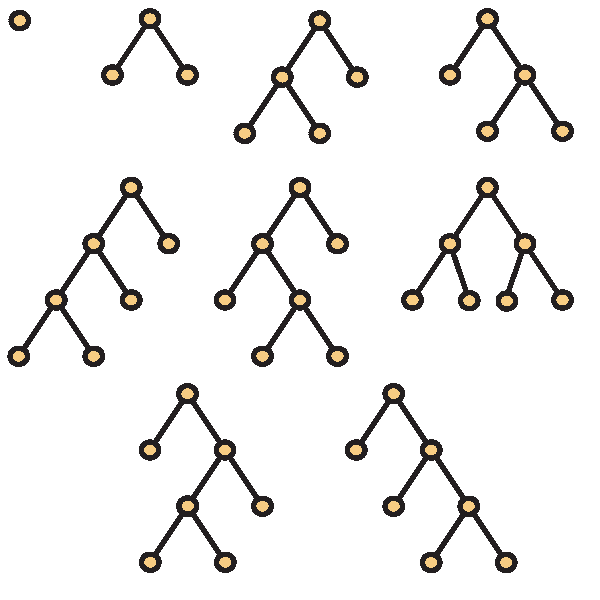
\includegraphics{recurrence-figs/RUBOTs}
  \caption{The RUBOTs with $n$ leaves for $n\leq 4$}
  \label{fig:rubots}
\end{figure}

Let $C(x) = \sum_{n=0}^\infty c_n x^n$ be the generating function for
the sequence $\{c_n\colon n\geq 0\}$ where $c_n$ is the number of
RUBOTs with $n$ leaves. (We take $c_0=0$ for convenience.) Then we can
see from \autoref{fig:rubots} that $C(x) = x + x^2 + 2x^3 + 5x^4 +
\cdots$. But what are the remaining coefficients? Let's see how we can
break a RUBOT with $n$ leaves down into a combination of two smaller
RUBOTs to see if we can express $c_n$ in terms of some $c_k$ for $k<
n$. When we look at a RUBOT with $n\geq 2$ leaves, we notice that the
root vertex must have two children. Those children can be viewed as
root nodes of smaller RUBOTs, say the left child roots a RUBOT with
$k$ leaves, meaning that the right child roots a RUBOT with $n-k$
leaves. Since there are $c_k$ possible sub-RUBOTs for the left child
and $c_{n-k}$ sub-RUBOTs for the right child, there are a total of
$c_kc_{n-k}$ RUBOTs in which the root's left child has $k$ leaves on
its sub-RUBOT. We can do this for any $k=1,2,\dots,n-1$, giving us
that
\[c_n = \sum_{k=1}^{n-1} c_kc_{n-k}.\]
(This is valid since $n\geq 2$.)
Since $c_0=0$, we can actually write this as
\[c_n = \sum_{k=0}^{n} c_kc_{n-k}.\]

Let's look at the square of the generating function $C(x)$. By
\hyperref[prop:genfunction-product]{Proposition~\ref*{prop:genfunction-product}},
we have
\begin{align*}
  C^2(x) &= c_0^2 + (c_0c_1 + c_1c_0)x + (c_0c_2 +c_1c_1 + c_2c_0)x^2 +
  \cdots\\
  & = 0 + 0 + (c_0c_2 +c_1c_1 + c_2c_0)x^2 + (c_0c_3 +
  c_1c_2+c_2c_1+c_3c_0)x^3 + \cdots.
\end{align*}
But now we see from our recursion above that the coefficient on $x^n$
in $C^2(x)$ is nothing but $c_n$ for $n\geq 2$. All we're missing is
the $x$ term, so adding it in gives us that
\[C(x) = x + C^2(x).\]
Now this is a quadratic equation in $C(x)$, so we can solve for $C(x)$
and have
\[C(x) = \frac{1\pm \sqrt{1-4x}}{2} = \frac{1\pm (1-4x)^{1/2}}{2} .\]
Hence, we can use \hyperref[thm:newton-binomial]{Newton's Binomial
  Theorem (\ref*{thm:newton-binomial})} to expand $C(x)$. To do so, we
use the following lemma. Its proof is nearly identical to that of
\hyperref[l:newbinom]{Lemma~\ref*{l:newbinom}}, and is thus omitted.

\begin{lemma}\label{l:half-binomial}
For each $k\ge 1$,
\[
\binom{1/2}{k}=\frac{(-1)^{k-1}}{k}\frac{\binom{2k-2}{k-1}}{2^{2k-1}}.
\]
\end{lemma}

Now we see that
\begin{align*}
  C(x) &= \frac{1}{2} \pm \frac{1}{2} \sum_{n=0}^\infty\binom{1/2}{n}
  (-4)^n x^n 
  = \frac{1}{2} \pm \frac{1}{2}\left(1+ \sum_{n=1}^\infty
\frac{(-1)^{n-1}}{n}\frac{\binom{2n-2}{n-1}}{2^{2n-1}}(-4)^n
x^n\right)\\
&=
\frac{1}{2} \pm\frac{1}{2} \mp\sum_{n=1}^\infty \frac{\binom{2n-2}{n-1}}{n} x^n.
\end{align*}
Since we need $c_n\geq 0$, we take the ``minus'' option from the
``plus-or-minus'' in the quadratic formula and thus have the following
theorem.

\begin{theorem}\label{thm:catalan-genfunction}
  The generating function for the number $c_n$ of rooted, unlabeled,
  binary, ordered trees with $n$ leaves is
  \[C(x) = \frac{1-\sqrt{1-4x}}{2} = \sum_{n=1}^\infty \frac{1}{n}\binom{2n-2}{n-1}x^n.\]
\end{theorem}

Notice that $c_n$ is a Catalan number, which we first encountered in
\autoref{ch:strings}, where we were counting lattice paths that did
not cross the diagonal line $y=x$. (The coefficient $c_n$ is the
Catalan number we called $C(n-1)$ in \autoref{ch:strings}.)

% As a consequence of \autoref{thm:catalan-genfunction}, we have the
% following corollary.

% \begin{corollary}\label{cor:2n-choose-n}
%   The generating functon of the sequence $\{\binom{2n}{n}:n\ge0\}$
%   is $f(x)=(1-4x)^{-1/2}$.
% \end{corollary}

% \begin{proof}
%   Differentiating $C(x)$ first as a function of $x$ and then as a
%   formal power series gives the desired result.
% \end{proof}

% Since the generating function $f(x)$ of
% \hyperref[cor:2n-choose-n]{Corollary~\ref*{cor:2n-choose-n}} squares
% to $1/(1-4x)$, we have the following corollary as a nice identity
% regarding binomial coefficients.

% \begin{corollary}
% For all $n\ge0$,
% \[
% 2^{2n}=\sum_{k=0}^n\binom{2k}{k}\binom{2n-2k}{k}.
% \]
% \end{corollary}

\section{Discussion}\label{s:recurrence:discussion}

Yolanda took a sip of coffee ``I'm glad I paid attention
when we were studying vector spaces, bases and dimension.
All this stuff about solutions for recurrence equations
made complete sense.   And I can really understand why
the professor was making a big deal out of factoring.
We saw it our first semester when we were learning about
partial fractions in calculus.  And we saw it again with the differential
equations stuff.  Isn't it really neat to see how it all
fits together.''  All this enthusiasm was too much for Alice who 
was not having a good day.  Bob was more sympathetic ``Except for
the detail about zero as a root of an advancement operator
polynomial, I was ok with this chapter.'' Xing said ``Here
we learned a precise approach that depended only on factoring.
I've been reading on the web and I see that there have
been some recent breakthroughs on factoring.''  Bob jumped
back in ``But even if you can factor like crazy, if you
have a large degree polynomial in the advancement operator
equation, then you will have lots of initial conditions.
This might be a second major hurdle.'' Dave mumbled ``Just
do the factoring. The rest is easy.''  Carlos again was
quiet but he knew that Dave was right.  Solving big
systems of linear equations is relatively easy. The
challenge is in the factoring stage.

\section{Exercises}\label{s:recurrence:exercises}

\begin{enumerate}
\item Write each of the following recurrence equations as advancement
  operator equations.
  \begin{multicols}{2}
    \begin{enumerate}
    \item $r_{n+2} = r_{n+1}+2r_n$
    \item $r_{n+4}=3r_{n+3} - r_{n+2}+2r_n$
    \item $g_{n+3} = 5 g_{n+1} - g_n + 3^n$
    \item $h_n = h_{n-1} - 2h_{n-2} + h_{n-3}$
    \item $r_n = 4r_{n-1} + r_{n-3} - 3 r_{n-5} + (-1)^n$
    \item $b_n = b_{n-1} + 3b_{n-2} + 2^{n+1} - n^2$
    \end{enumerate}
  \end{multicols}
\item Solve the recurrence equation $r_{n+2} = r_{n+1} + 2r_n$ if
  $r_0=1$ and $r_2=3$ (Yes, we specify a value for $r_2$ but not for
  $r_1$).
\item Find the general solution of the recurrence equation $g_{n+2} =
  3g_{n+1}-2g_n$.
\item Solve the recurrence equation $h_{n+3} = 6h_{n+2}-11h_{n+1} +
  6h_n$ if $h_0=3$, $h_1=2$, and $h_2=4$.
\item Find an explicit formula for the $n^\text{th}$ Fibonacci number
  $f_n$. (See \autoref{s:recurrence:intro:fib}.)
\item For each advancement operator equation below, give its general
  solution.
  \begin{multicols}{2}
    \begin{enumerate}
    \item $(A-2)(A+10)f=0$
    \item $(A^2-36)f=0$
    \item $(A^2-2A-5)f=0$
    \item $(A^3-4 A^2-20 A+48)f=0$
    \item $(A^3 +A^2-5A+ 3)f=0$
    \item $(A^3+3 A^2+3 A+1)f=0$
    \end{enumerate}
 \end{multicols}
\item Solve the advancement operator equation $(A^2+3 A-10)f=0$ if
  $f(0)=2$ and $f(1)=10$.
\item Give the general solution to each advancement operator equation
  below.
  \begin{enumerate}
  \item $(A-4)^3(A+1)(A-7)^4(A-1)^2 f =0$
  \item $(A+2)^4(A-3)^2(A-4)(A+7)(A-5)^3g=0$
  \item $(A-5)^2(A+3)^3(A-1)^3(A^2-1)(A-4)^3h=0$
  \end{enumerate}
\item For each nonhomogeneous advancement operator equation, find its
  general solution.
  \begin{multicols}{2}
    \begin{enumerate}
    \item $(A-5)(A+2)f=3^n$
    \item $(A^2+3A-1)g = 2^n + (-1)^n$
    \item $(A-3)^3 f = 3n+1$
    \item $(A^2+3A-1)g = 2n$
    \item $(A-2)(A-4)f=3n^2 + 9^n$
    \item $(A+2)(A-5)(A-1)f = 5^n$
    \item $(A-3)^2(A+1)g=  2\cdot 3^n$
    \item $(A-2)(A+3)f=5n2^n$
    \item $(A-2)^2(A-1)g=3n^22^n + 2^n$
    \item $(A+1)^2(A-3)f = 3^n + 2n^2$
    \end{enumerate}
  \end{multicols}
\item Find and solve a recurrence equation for the number $g_n$ of
  ternary strings of length $n$ that do not contain $102$ as a
  substring. 
\item There is a famous puzzle called the Towers of Hanoi that
  consists of three pegs and $n$ circular discs, all of different
  sizes. The discs start on the leftmost peg, with the largest disc on
  the bottom, the second largest on top of it, and so on, up to the
  smallest disc on top. The goal is to move the discs so that they are
  stacked in this same order on the rightmost peg. However, you are
  allowed to move only one disc at a time, and you are never able to
  place a larger disc on top of a smaller disc. Let $t_n$ denote the
  fewest moves (a move being taking a disc from one peg and placing it
  onto another) in which you can accomplish the goal. Determine an
  explicit formula for $t_n$.
\item A valid database identifier of length $n$ can be
  constructed in three ways:
  \begin{itemize}
  \item Starting with $A$ and followed by any valid identifier of
    length $n-1$.
  \item Starting with one of the two-character strings $1A$, $1B$,
    $1C$, $1D$, $1E$, or $1F$ and followed by any valid identifier of
    length $n-2$.
  \item Starting with $0$ and followed by any ternary ($\{0,1,2\}$)
    string of length $n-1$.
  \end{itemize}
  Find a recurrence for the number $g(n)$ of database identifiers of
  length $n$ and then solve your recurrence to obtain an explicit
  formula for $g(n)$. (You may consider the empty string of length $0$
  a valid database identifier, making $g(0)=1$. This will simplify the
  arithmetic.)
\item Let $t_n$ be the number of ways to tile a $2\times n$ rectangle
  using $1\times 1$ tiles and $L$-tiles. An $L$-tile is a $2\times 2$
  tile with the upper-right $1\times 1$ square deleted. (An $L$ tile
  may be rotated so that the ``missing'' square appears in any of the
  four positions.) Find a recursive formula for $t_n$ along with
  enough initial conditions to get the recursion started. Use this
  recursive formula to find a closed formula for $t_n$.
\item Prove \hyperref[lem:rr]{Lemma~\ref*{lem:rr}} about advancement
  operator equations with repeated roots.
\item Use generating functions to solve the recurrence equation
  $r_n=4r_{n-1}+6r_{n-2}$ for $n\geq 2$ with $r_0=1$ and $r_1=3$.
\item Let $a_0=0$, $a_1=2$, and $a_2=5$. Use generating functions to
  solve the recurrence equation $a_{n+3} = 5a_{n+2} - 7a_{n+1}+3a_n +
  2^n$ for $n\geq 0$.
\item Let $b_0=1$, $b_2=1$, and $b_3=4$. Use generating functions to
  solve the recurrence equation $b_{n+3} = 4b_{n+2}-b_{n+1}-6b_n +
  3^n$ for $n\geq 0$.
\item Use generating functions to find a closed formula for the
  Fibonacci numbers $f_n$. 
\item How many rooted, unlabeled, binary, ordered, trees (RUBOTs) with
  $6$ leaves are there? Draw $6$ distinct RUBOTs with $6$ leaves.
\item In this chapter, we developed a generating function for the
  Catalan numbers. We first encountered the Catalan numbers in
  \autoref{ch:strings}, where we learned they count certain lattice
  paths. Develop a recurrence for the number $l_n$ of lattice paths
  similar to the recurrence
  \[c_n = \sum_{k=0}^n c_k c_{n-k}\qquad \text{for }n\geq 2\]
  for RUBOTs by thinking of ways to break up a lattice path from
  $(0,0)$ to $(n,n)$ that does not cross the diagonal $y=x$ into two
  smaller lattice paths of this type.

\end{enumerate}

%%% Local Variables: 
%%% mode: latex
%%% TeX-master: "chap-skel-mtk"
%%% End: 
